\documentclass[12pt,letterpaper]{article}

\usepackage[utf8]{inputenc}
\usepackage[T1]{fontenc}
\usepackage{amsmath}
\usepackage{amsfonts}
\usepackage{amssymb}
\usepackage{amsthm}
\usepackage[left=2cm,right=2cm,top=2cm,bottom=2cm,headheight=22pt]{geometry}
\usepackage{fancyhdr}
\usepackage{setspace}
\usepackage{lastpage}
\usepackage{graphicx}
\usepackage{caption}
\usepackage{subcaption}


\theoremstyle{definition}
\newtheorem{question}{Question}
\newtheorem{example}{Example}
\newtheorem{exercise}[question]{Exercise}
\newtheorem*{challenge}{Challenge}

\begin{document}

%Paramètres de mise en forme des paragraphes selon les normes françaises
\setlength{\parskip}{1ex plus 0.5ex minus 0.2ex}
\setlength{\parindent}{0pt}

%Paramètres relatifs aux en-têtes et pieds de page.
\pagestyle{fancy}
\lhead{Theron J Hitchman}
\chead{\Large Meeting 10}
\rhead{Fall 2013}
\lfoot{\emph{Math and Decision Making}}
\cfoot{}
\rfoot{\emph{\thepage\ of \pageref{LastPage}}}


\section*{Reidemeister Moves of Type III and tricolorability}

How does a Reidemeister move of type III affect the tricolorability of a knot or link?
It turns out, \emph{not at all}. That is, if two planar projections differ by just one Reidemeister move of type III, then thoes two projections are either both tricolorable, or both not tricolorable. 

How can we understand this to be true? 
The simplest way is to just check it directly.
We will make a list of all the possible tricolorings of a three crossing arrangment where a type III move might be made, and check that after the move, the knot is still tricolorable.

Recall that the diagram change involved in a Reidemeister move of type III is this one:

\begin{figure}[h]
    \centering
    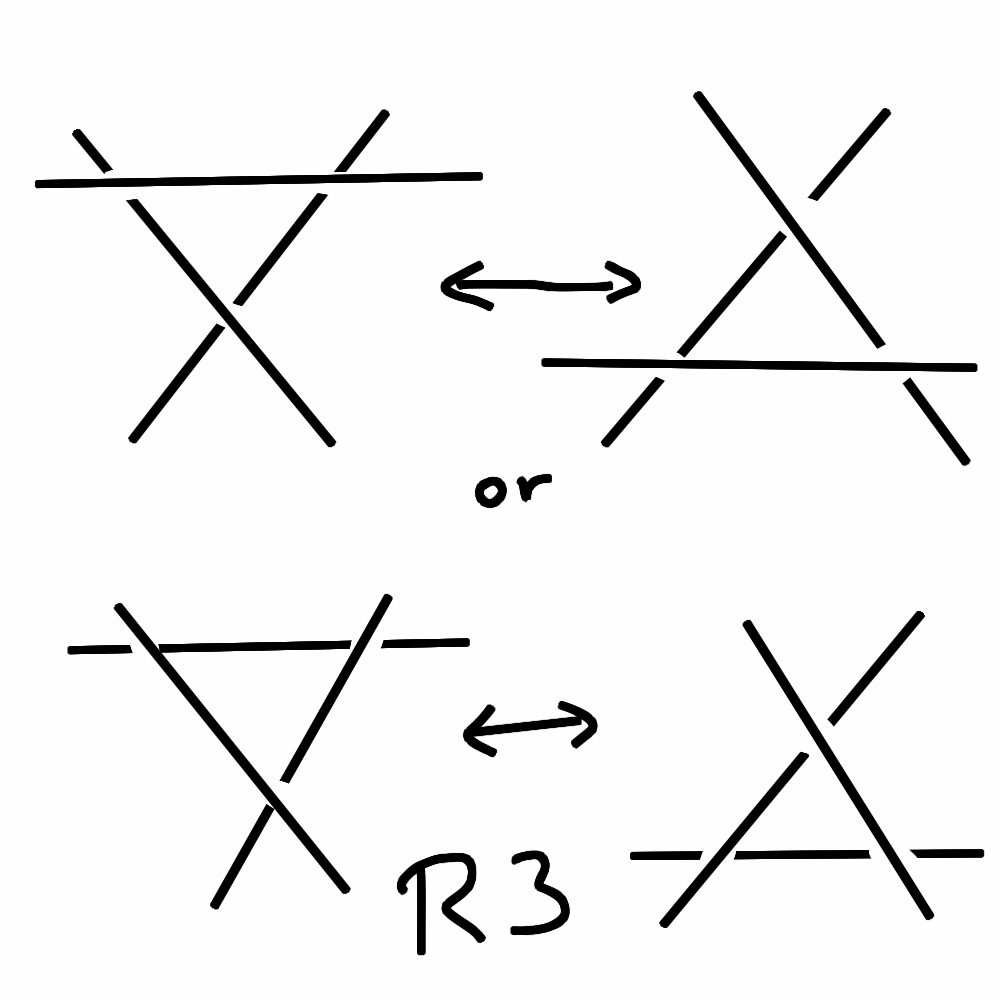
\includegraphics[width=.4\textwidth]{meeting10pics/r3.png}
    \caption{Type III Reidemeister move.}
\end{figure}

How many ways are there to color the strands in this figure?
Many, I suppose.
But the crucial thing is that the colors are either the same or different at each crossing.
There are three crossings here, and at each one, there two choices (all the same color or all different colors).
This means there should be no more than $2\times 2 \times 2 = 8$ essentially different colorings.

(What do we mean by ``essentially different colorings?" Well, swapping out the names of the colors really shouldn't change the type of the argument here. So, we can decide to change all of the red strands for blue strands and vice versa, leaving all of the green strands alone, and we would get basically the same logic even though the colors are technically in different places.)

The other thing to be wary about is that a coloring has to satisfy the basic rules, but since strands in one crossing are also in the other crossings, the choices aren't completely independent. This reduces the number of options we really have to consider.
In the end, there are only five.

Now we list all of the possible ways to make essentially different colorings of the type three diagram, and show how after a Reidemeister move of type III the new diagram is still tricolorable.

Label the crossings 1, 2, and 3 from the upper left going clockwise.
We will organize things by what happens at the crossings.

\clearpage

\subsection*{The Pictures}
Note that it is important that the ``ends'' don't change colors as we perform the switch. 
Each end is attached to some strand of the knot, which has a color.
It cannot be allowed to change without messing up the coloring of the rest of the knot or link.

\begin{figure}[h!]
    \centering
    \begin{subfigure}{.4\textwidth}
        \centering
        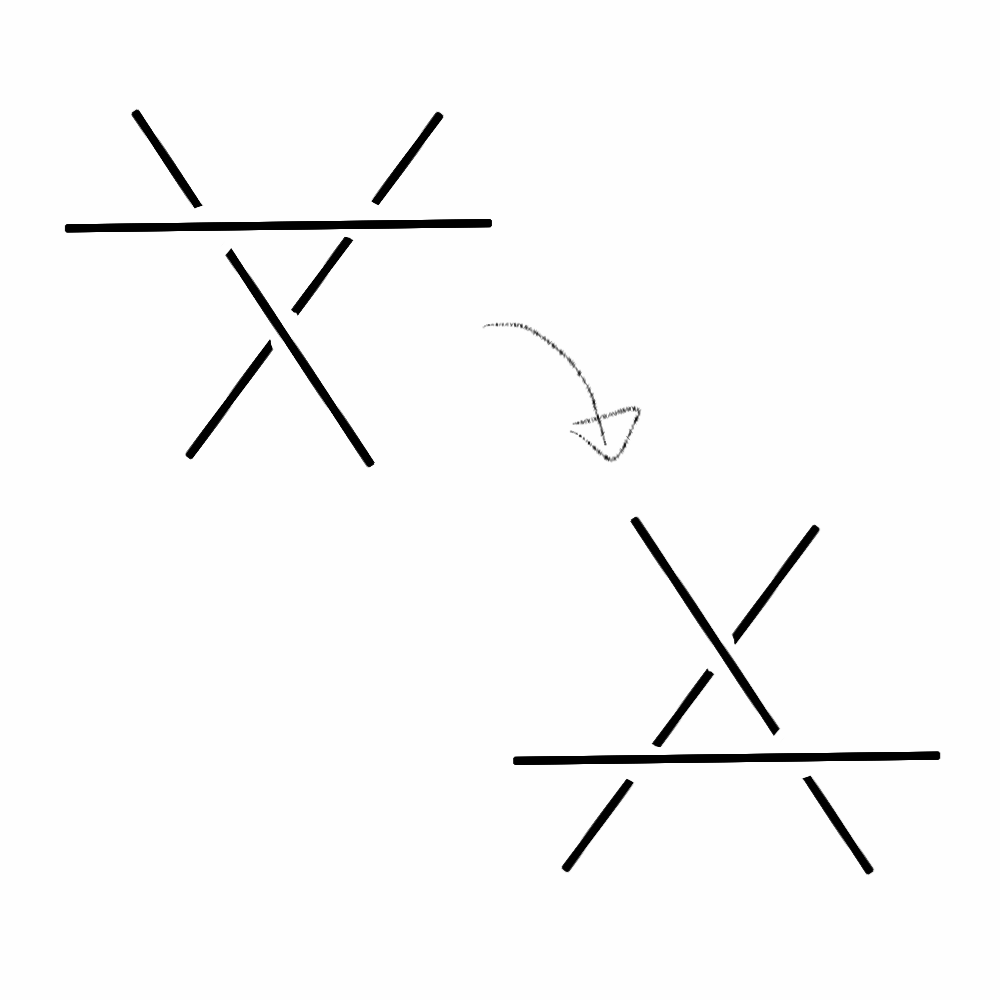
\includegraphics[width=\textwidth]{meeting10pics/1s2s.png}
        \caption{1 \& 2 all the same, 3 is forced}
    \end{subfigure}
    \qquad
    \begin{subfigure}{.4\textwidth}
        \centering
        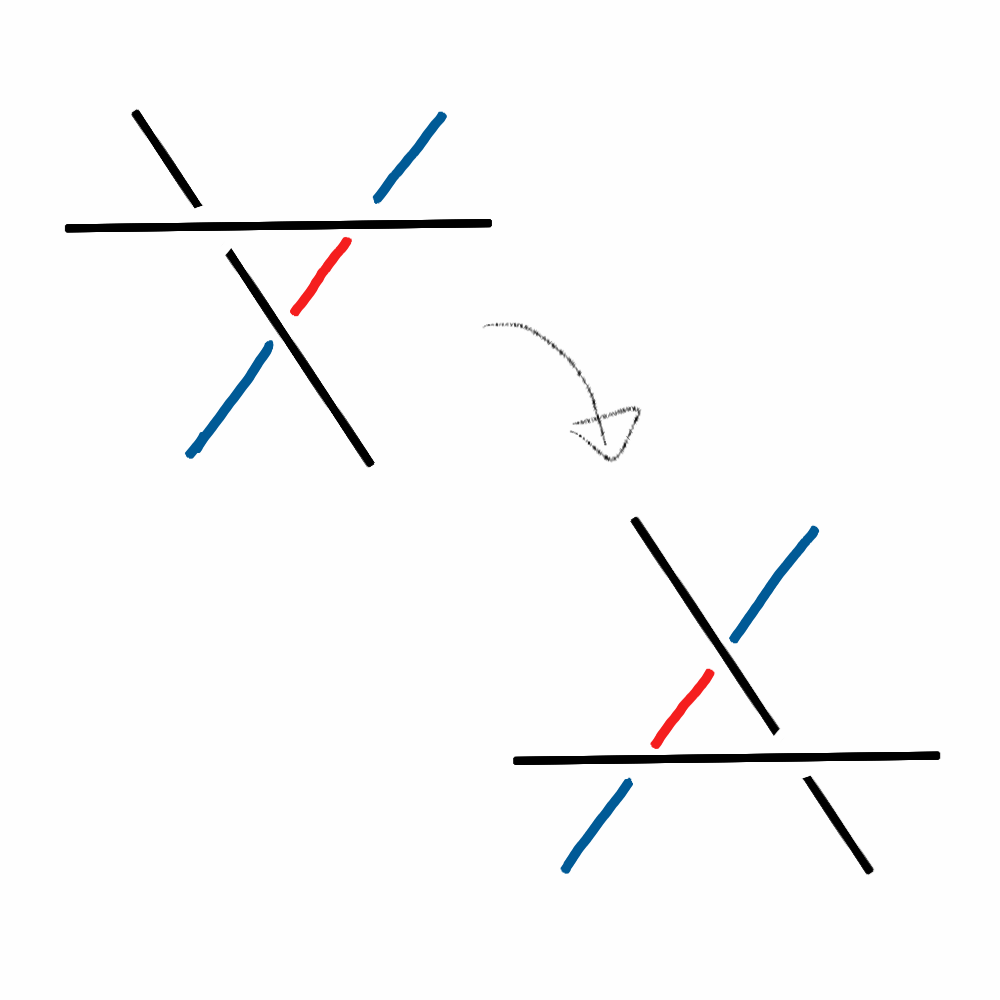
\includegraphics[width=\textwidth]{meeting10pics/1s2d.png}
        \caption{1 all the same, 2 all different, 3 is forced}
    \end{subfigure}
    \caption{Possibilities with crossing 1 all the same color}
\end{figure}

\begin{figure}[h!]
    \centering
    \begin{subfigure}{.3\textwidth}
        \centering
        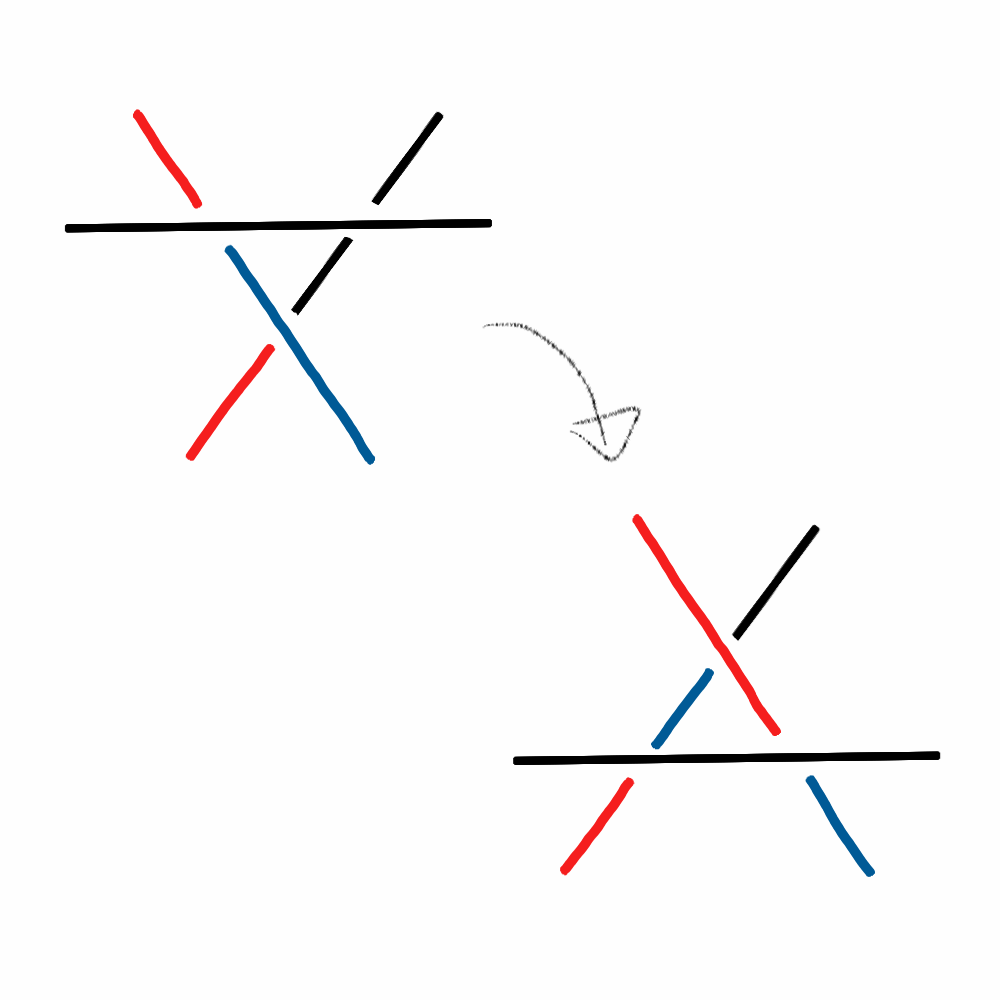
\includegraphics[width=\textwidth]{meeting10pics/1d2s.png}
        \caption{1 different, 2 same, 3 forced}
    \end{subfigure}
    \quad
    \begin{subfigure}{.3\textwidth}
        \centering
        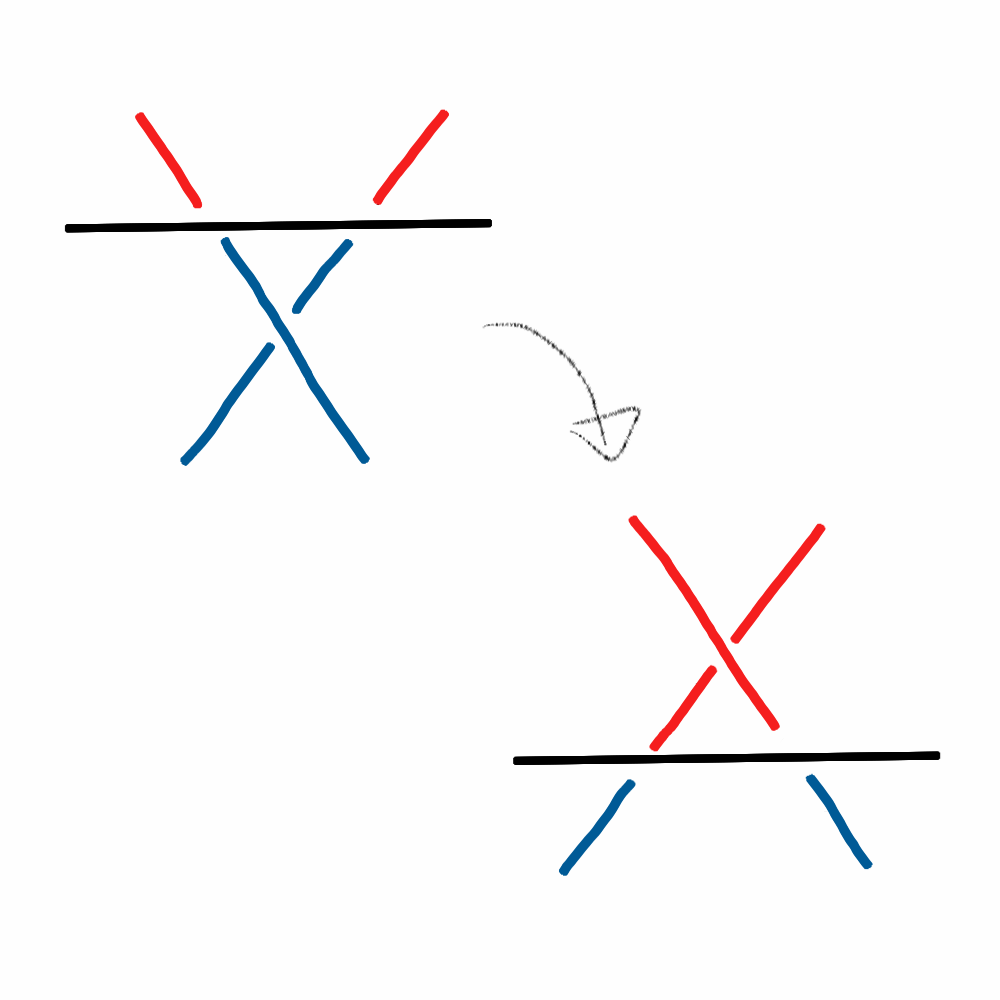
\includegraphics[width=\textwidth]{meeting10pics/1d2d3s.png}
        \caption{1 same, 2 different, 3 same}
    \end{subfigure}
    \quad
    \begin{subfigure}{.3\textwidth}
        \centering
        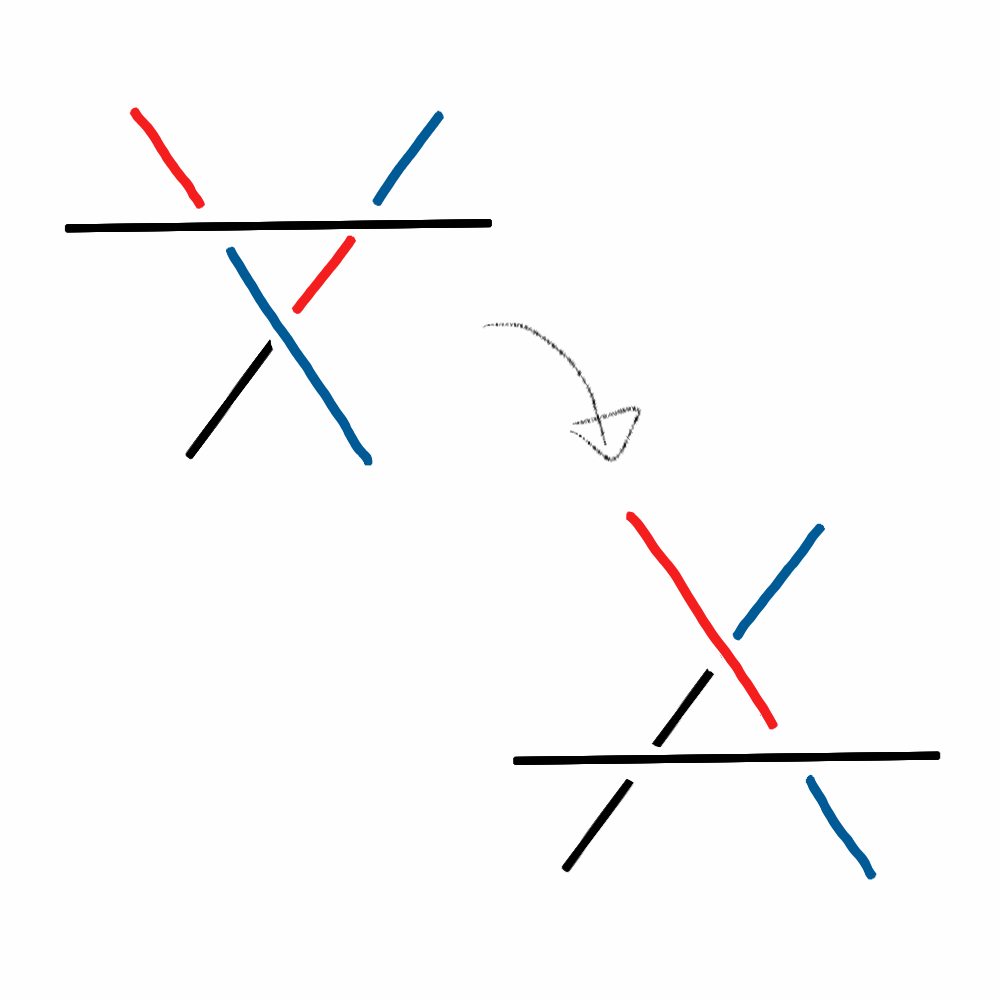
\includegraphics[width=\textwidth]{meeting10pics/1d2d3d.png}
        \caption{1 same, 2 \& 3 different}
    \end{subfigure}
    \caption{Possibilities with crossing 1 all different colors}
\end{figure}



\end{document}